\part{Diagramme de collaboration - Validation de l'architecture globale}
\setcounter{section}{0}

\section{Diagramme de collaboration}
\begin{figure}[H]
\noindent\makebox[\textwidth]{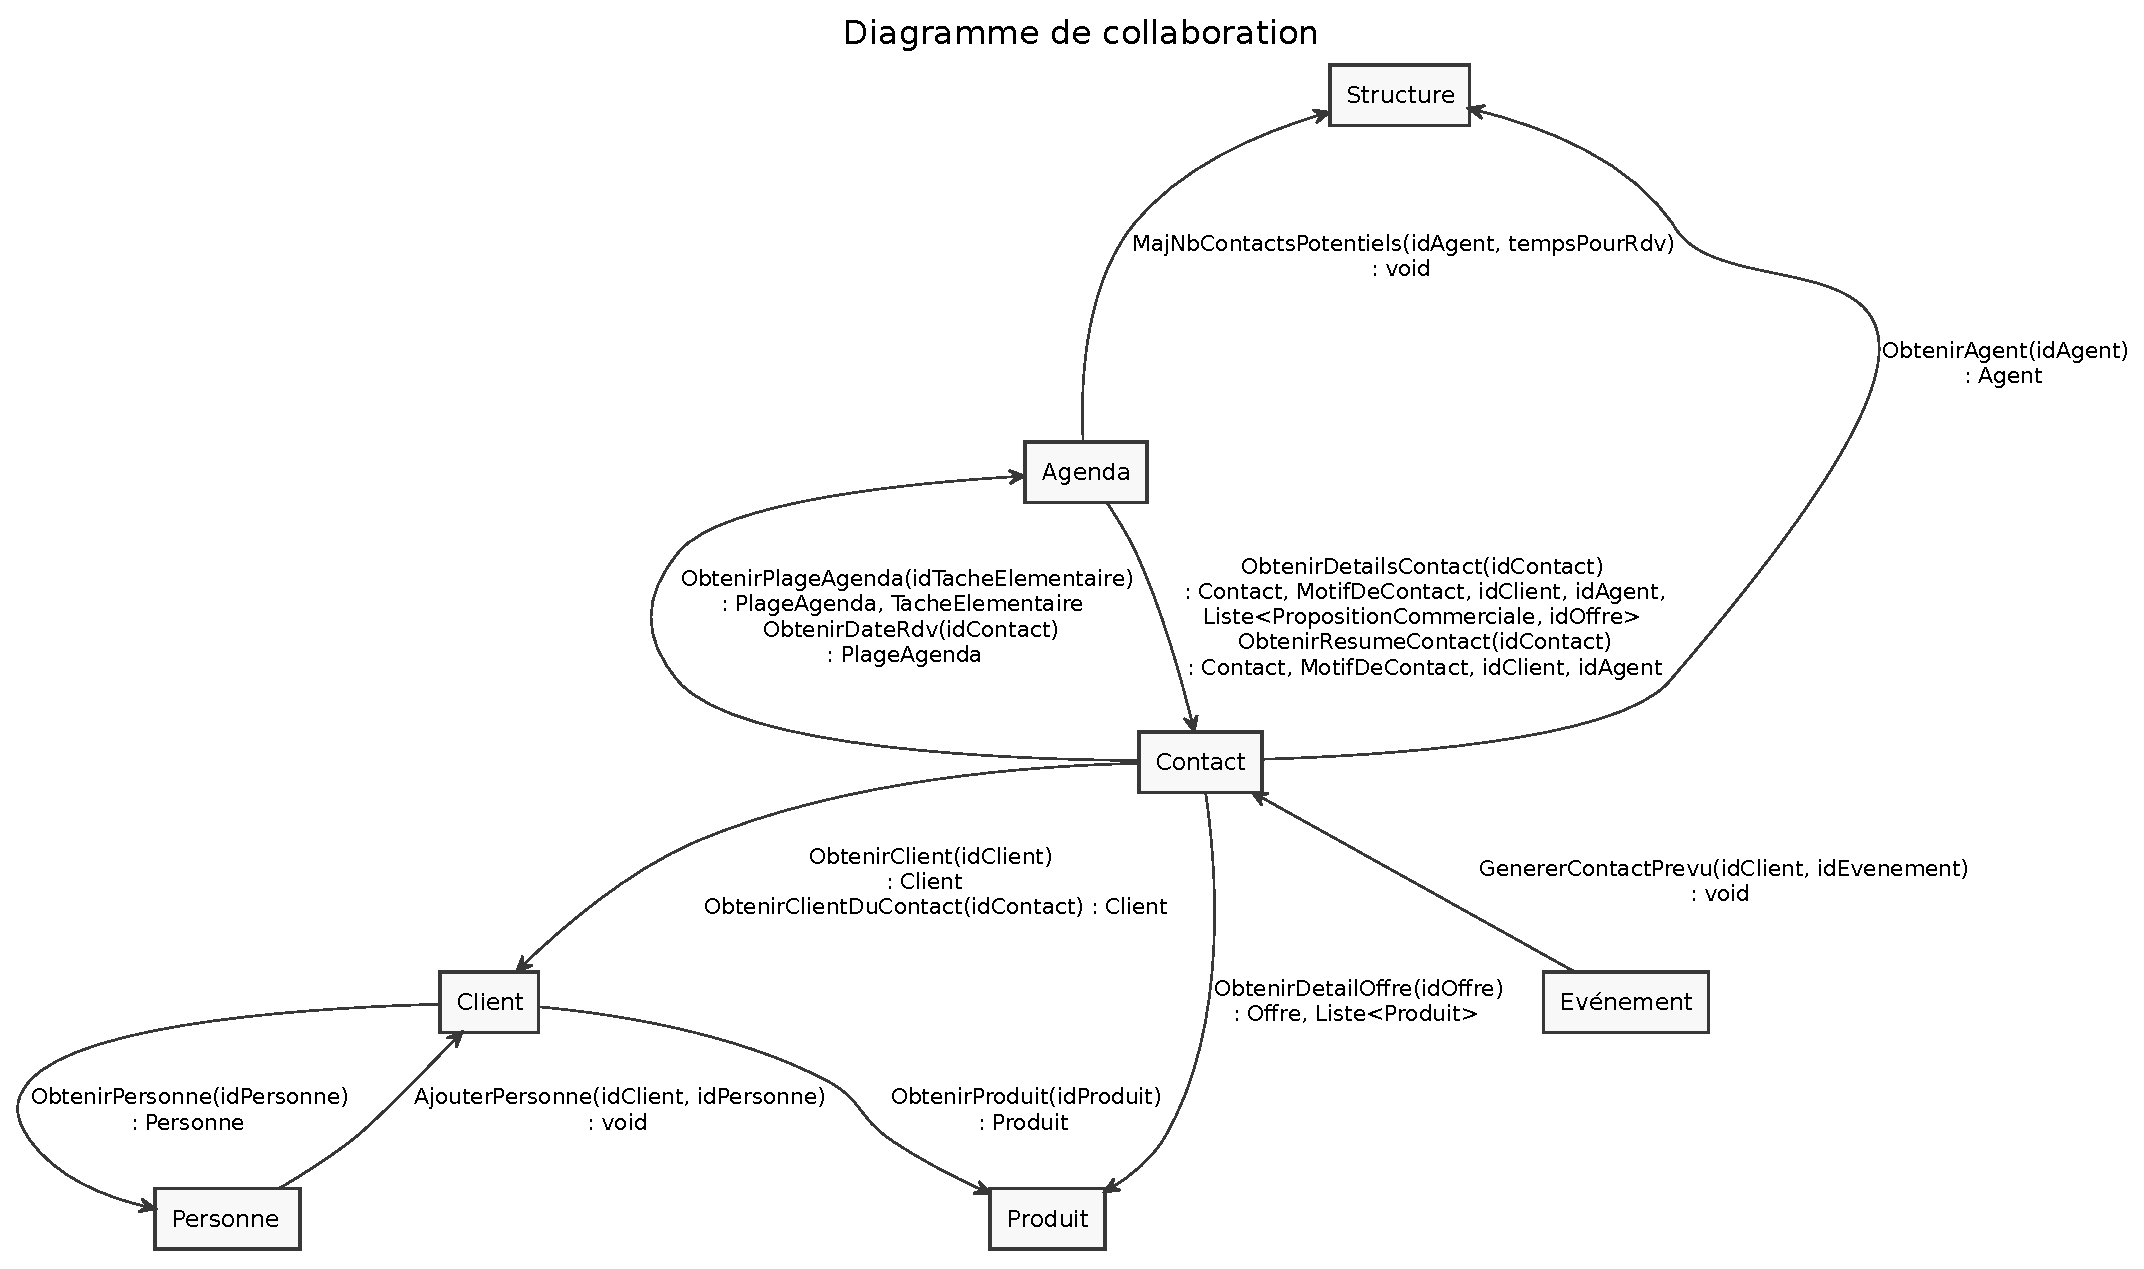
\includegraphics[width=23cm, angle=90]{figures/eps/collaboration.eps}}
\caption{Diagramme de collaboration}
\end{figure}

Nous pouvons constater que la répartition des services entre les blocs est centrée autour de l'objet contact. S'agissant du cœur de métier du projet, nous pouvons en déduire que nos choix de découpage en blocs ont été correctement fondés. En effet, la répartition des différents appels semble être assez homogène et nous n'observons pas de redondances. \\

Nous pouvons également observer qu'il n'y a pas de croisements entre tous les blocs, déterminant ainsi des groupements de blocs plus généraux. Il s'agit principalement de services de consultation, les services de modification restant minoritaires.\\

Enfin, nous retrouvons les différents liens établies dans le MCB. Par exemple, nous avons bien le lien entre le bloc Contact et Client, qui représente l'ensemble des associations effectuées entre les entités de ces deux blocs.



